\documentclass[conference]{IEEEtran}

\usepackage[utf8]{inputenc}
\usepackage[T1]{fontenc}
\usepackage[english]{babel}
\usepackage{amsmath}
\usepackage{booktabs}
\usepackage{cite}
\usepackage{graphicx}
\usepackage{hyperref}
\usepackage{url}

\title{Prediction and Analysis of Academic Performance Using Artificial Intelligence}

\author{
\IEEEauthorblockN{Edson Manuel Zepeda Chavez}
\IEEEauthorblockA{\textit{Samsung Innovation Campus 2025--2026}\\
\textit{Universidad de Colima, Bachillerato 16}\\
rmcedson09@gmail.com}
\and
\IEEEauthorblockN{Francisco Ricardo Moreno Sanchez}
\IEEEauthorblockA{\textit{Samsung Innovation Campus 2025--2026}\\
\textit{CONALEP Plantel 262}\\
fmorenosanchez39@gmail.com}
\and
\IEEEauthorblockN{Alan Emir Martinez Espinosa}
\IEEEauthorblockA{\textit{Samsung Innovation Campus 2025--2026}\\
\textit{CONALEP Plantel 262}\\
maresesp012@gmail.com}
}

\newcommand{\projectlogos}{%
\begin{center}
\IfFileExists{figures/logo_udem.png}{
\includegraphics[height=0.8cm]{figures/logo_udem.png}\hspace{1.2cm}}{}%
\IfFileExists{figures/logo_sic.png}{
\includegraphics[height=0.8cm]{figures/logo_sic.png}}{}%
\end{center}
}

\begin{document}
\maketitle
\projectlogos

\begin{abstract}
This article presents a predictive and interpretable system for estimating student academic performance and translating model outputs into actionable early-intervention recommendations. The study uses a tabular dataset of 2,392 students and 15 variables, including age, weekly study time, absences, tutoring, parental support, extracurricular activities, and GPA. The proposed approach combines two complementary tasks: a regression task to estimate GPA and a calibrated classification task to estimate the probability of achieving good academic performance, defined as GPA $\geq 2.5$. LinearRegression, Random Forest, SVR, and XGBoost were compared. The best regression model was LinearRegression, with RMSE = 0.1963 and $R^2$ = 0.9534 on the test set. XGBoost produced predictions highly similar to those of the linear model, with a correlation of 0.9957, but it showed a larger train-test gap and therefore did not generalize better. An ablation test removing the Absences variable increased the linear model RMSE from 0.1963 to 0.8692, confirming that absences are the dominant factor in the dataset. Finally, a recommendation engine was implemented to simulate feasible interventions, exclude sensitive or non-actionable variables, and prioritize actions by their estimated impact on GPA and probability of good performance. The results suggest that the practical value of the system is not only prediction, but the conversion of predictive outputs into supervised support for students and tutors.
\end{abstract}

\begin{IEEEkeywords}
academic performance, GPA, machine learning, Educational Data Mining, XGBoost, academic recommendations, early warning, interpretability.
\end{IEEEkeywords}

\section{Introduction}

Early prediction of academic performance is a relevant application of Educational Data Mining because it can help identify at-risk students and guide support resources before low performance becomes consolidated. Recent literature shows that machine learning models can be useful for anticipating academic outcomes and supporting educational decisions \cite{khairy2024prediction}. However, a system that only returns a label or score has limited practical value: for a school, tutor, or student, the key question is not only ``what GPA is expected'', but also ``what can be improved to increase the probability of good performance''.

This work addresses that problem through a reproducible workflow that combines prediction, interpretation, and recommendation. First, a set of regression models is trained to estimate GPA. Second, the behavior of XGBoost is analyzed to explain why it does not outperform the linear model even though their predictions are very similar. Third, an ablation test is performed by removing Absences to measure the dependency of the model on that variable. Fourth, a calibrated classifier is trained to estimate the probability of good performance, defined as GPA $\geq 2.5$. Fifth, a recommendation engine is built to test intervention scenarios over actionable variables.

The main contribution of this article is a practical path for turning an academic performance prediction model into a decision-support tool. The proposal avoids recommending changes based on sensitive or non-modifiable variables, such as Gender, Ethnicity, StudentID, and GradeClass, and instead focuses on variables where an educational intervention can be meaningful: absences, study time, tutoring, parental support, and participation in activities. This distinction is important because educational models can create risks of bias or misuse if they are transformed into automated decisions without human supervision \cite{hardt2016equality,barocas2023fairness}.

\section{Related Work}

The use of classification and regression models to estimate student performance is a consolidated topic in Educational Data Mining. Khairy et al. \cite{khairy2024prediction} show that data mining algorithms can support the prediction of exam performance. Other studies compare models such as Decision Tree, Random Forest, KNN, Naive Bayes, and SVM for academic performance prediction, with the goal of supporting early warning systems and intervention programs. In parallel, methods such as Random Forest \cite{breiman2001random}, Support Vector Machines \cite{cortes1995support}, and XGBoost \cite{chen2016xgboost} have been widely used because of their ability to model nonlinear relationships and capture interactions.

The gap addressed by this project is not merely obtaining a high metric, but connecting predictive outputs with interpretable actions. A model with strong performance can still be of limited use if it does not translate its output into understandable and actionable recommendations. Therefore, this work incorporates a simple counterfactual module: it modifies actionable variables, recomputes the estimated GPA, and recomputes the probability of good performance to prioritize improvement plans.

\section{Data}

The local file \texttt{student\_performance.csv} was used. The dataset source is Kaggle, ``Students Performance Dataset'', by Rabie El Kharoua \cite{kharoua2024students}. The local file matches the expected schema: 2,392 records and 15 columns.

The available columns are StudentID, Age, Gender, Ethnicity, ParentalEducation, StudyTimeWeekly, Absences, Tutoring, ParentalSupport, Extracurricular, Sports, Music, Volunteering, GPA, and GradeClass. No missing values were observed. The GPA observed in the local file ranges from 0.0 to 4.0, with a mean of 1.9062. To build the classification target, good performance was defined as GPA $\geq 2.5$, resulting in 706 students in the positive class and 1,686 below the threshold.

\begin{figure}[!t]
\centering
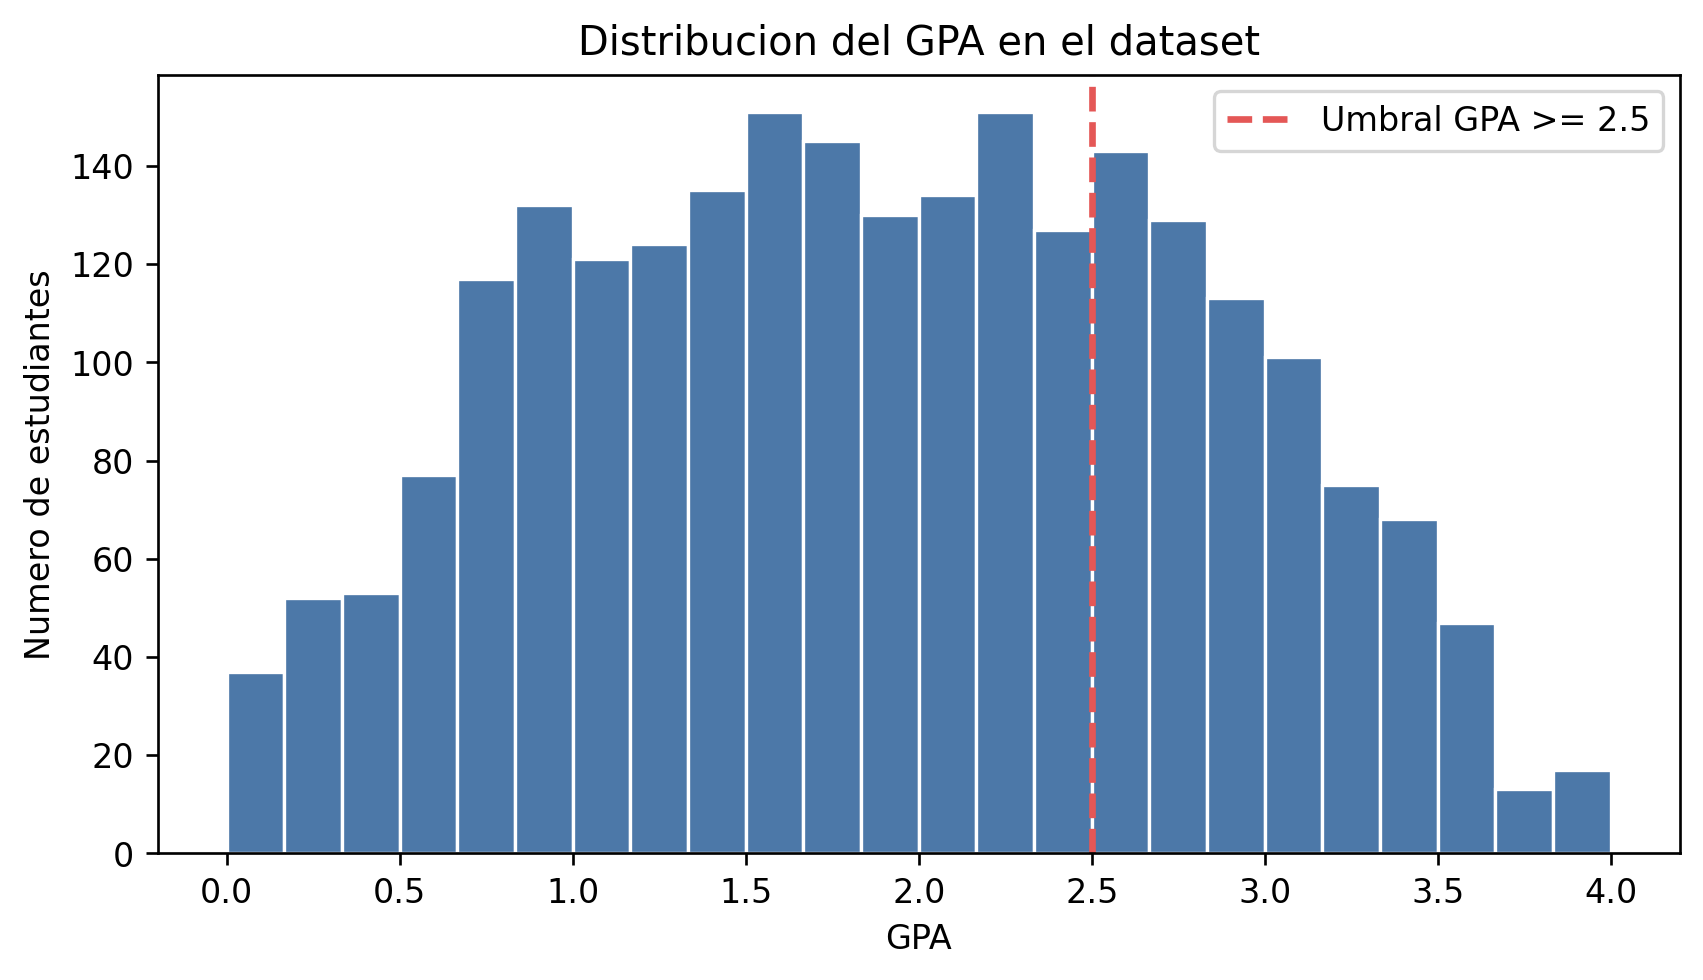
\includegraphics[width=\linewidth]{figures/fig_gpa_distribution.png}
\caption{Distribution of observed GPA and the threshold used to define good performance.}
\label{fig:gpa_distribution}
\end{figure}

\begin{figure}[!t]
\centering
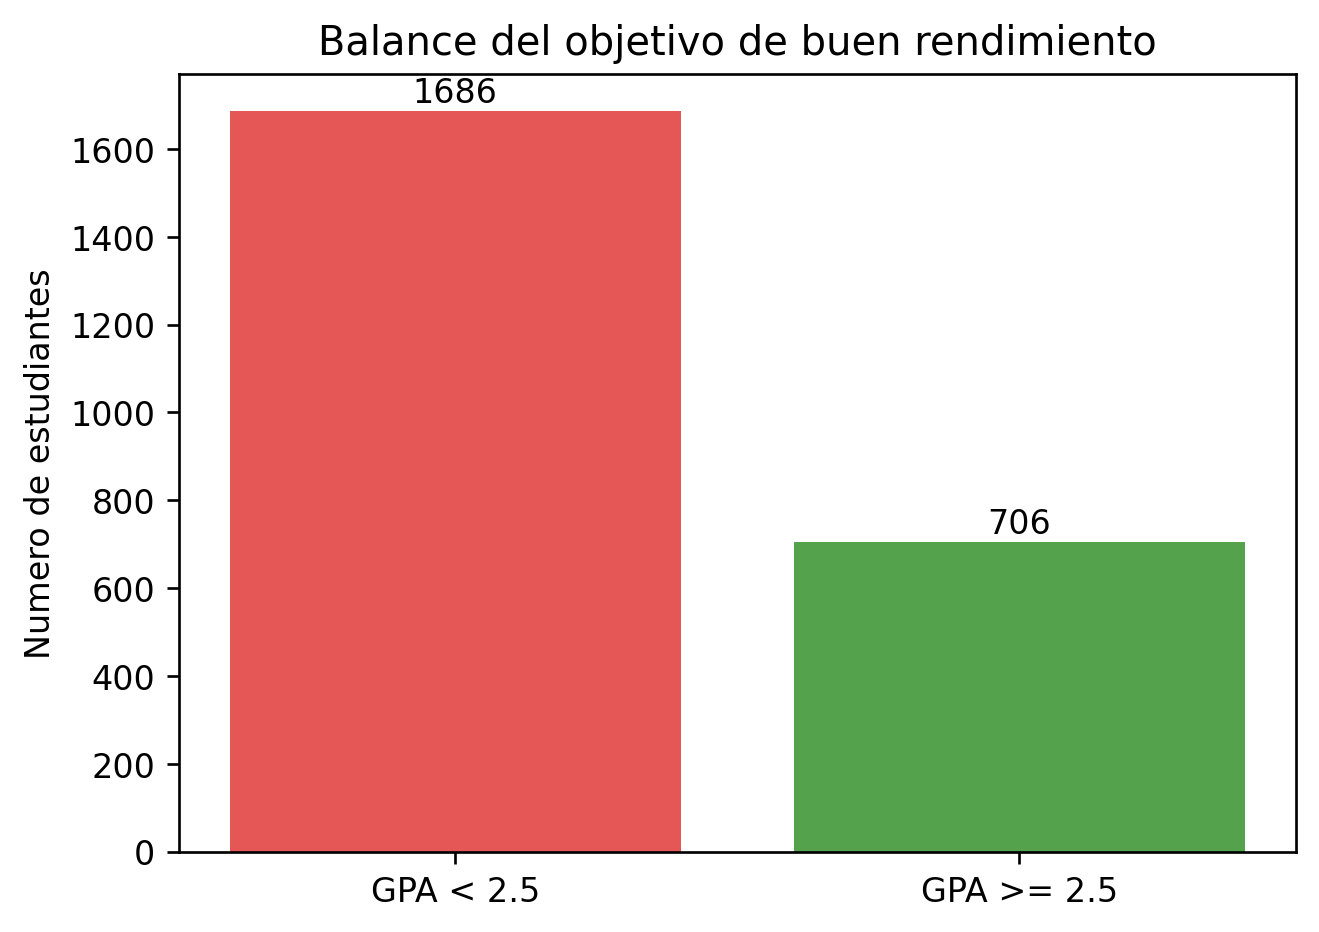
\includegraphics[width=.78\linewidth]{figures/fig_good_performance_balance.png}
\caption{Class balance for the good-performance classifier.}
\label{fig:class_balance}
\end{figure}

\section{Methodology}

\subsection{Data Preparation}

For the regression task, GPA was used as the target variable and StudentID and GradeClass were removed. StudentID is an identifier with no generalizable predictive value, while GradeClass directly encodes performance; using it to predict GPA would introduce data leakage. Demographic variables encoded in the dataset were retained for the general predictive analysis, but they were excluded from the recommendation engine.

Preprocessing was implemented with scikit-learn pipelines \cite{pedregosa2011scikit}. Numeric variables were imputed with the median and scaled with StandardScaler. Encoded categorical variables were imputed with the most frequent value and transformed with OneHotEncoder. The dataset was split into training and test sets using an 80/20 split and \texttt{random\_state = 42}. Stability was assessed with 5-fold cross-validation.

\subsection{Regression Models}

Four models were trained to estimate GPA: LinearRegression, RandomForestRegressor, SVR with an RBF kernel, and XGBRegressor. The main evaluation metrics were MAE, RMSE, and $R^2$. RMSE was selected as the main comparison metric because it penalizes large GPA errors, which is relevant in early-warning settings.

\subsection{XGBoost Analysis and Ablation}

XGBoost was analyzed specifically because its results were close to those of the linear model, but not superior. Training, test, and cross-validation metrics were compared. In addition, the correlation between LinearRegression and XGBoost predictions was measured. To study the model dependency on absences, training was repeated after removing Absences and the resulting RMSE was compared with the baseline.

\subsection{Good-Performance Classifier}

To generate messages such as ``this increases your probability of good performance'', a second classification task was trained. The target variable was defined as:

\begin{equation}
y_{good} =
\begin{cases}
1, & \text{if } GPA \geq 2.5\\
0, & \text{if } GPA < 2.5
\end{cases}
\end{equation}

LogisticRegression, RandomForestClassifier, HistGradientBoostingClassifier, and XGBClassifier were evaluated. The best classifier was selected by cross-validated ROC AUC and later calibrated with CalibratedClassifierCV using sigmoid calibration. Calibration was included because the recommendation engine uses probabilities to compare scenarios, not only binary classes.

\subsection{Recommendation Engine}

The recommendation engine uses only actionable or non-sensitive contextual variables: Age, StudyTimeWeekly, Absences, ParentalEducation, Tutoring, ParentalSupport, Extracurricular, Sports, Music, and Volunteering. StudentID, GradeClass, Gender, and Ethnicity are excluded. The simulated interventions include reducing absences, increasing study hours, enabling tutoring, increasing parental support, and enabling a complementary activity. For intensive scenarios, the engine also considers reducing absences to a maximum of 5 and increasing study time up to 20 weekly hours.

For each plan, the system computes the current estimated GPA, post-intervention estimated GPA, current probability of good performance, post-intervention probability, and expected difference. Plans are ranked by probability increase, GPA increase, and estimated effort. Outputs from the support regressor are clipped to the valid GPA range [0, 4] to avoid impossible messages in extreme cases.

\section{Results}

\subsection{GPA Regression}

\begin{table}[!t]
\centering
\caption{Comparison of regression models for GPA prediction.}
\label{tab:regression}
\begin{tabular}{lrrrrr}
\toprule
Model & MAE & RMSE & $R^2$ & CV RMSE & CV $R^2$ \\
\midrule
LinearRegression & 0.1551 & 0.1963 & 0.9534 & 0.1974 & 0.9533 \\
XGBoost & 0.1656 & 0.2117 & 0.9458 & 0.2138 & 0.9452 \\
SVR RBF & 0.2024 & 0.2520 & 0.9232 & 0.2491 & 0.9257 \\
Random Forest & 0.1964 & 0.2529 & 0.9226 & 0.2460 & 0.9275 \\
\bottomrule
\end{tabular}
\end{table}

LinearRegression obtained the best test performance, with RMSE = 0.1963 and $R^2$ = 0.9534. Cross-validation was consistent, with CV RMSE = 0.1974 and CV $R^2$ = 0.9533. This indicates that the result does not depend only on a favorable test split.

\begin{figure}[!t]
\centering
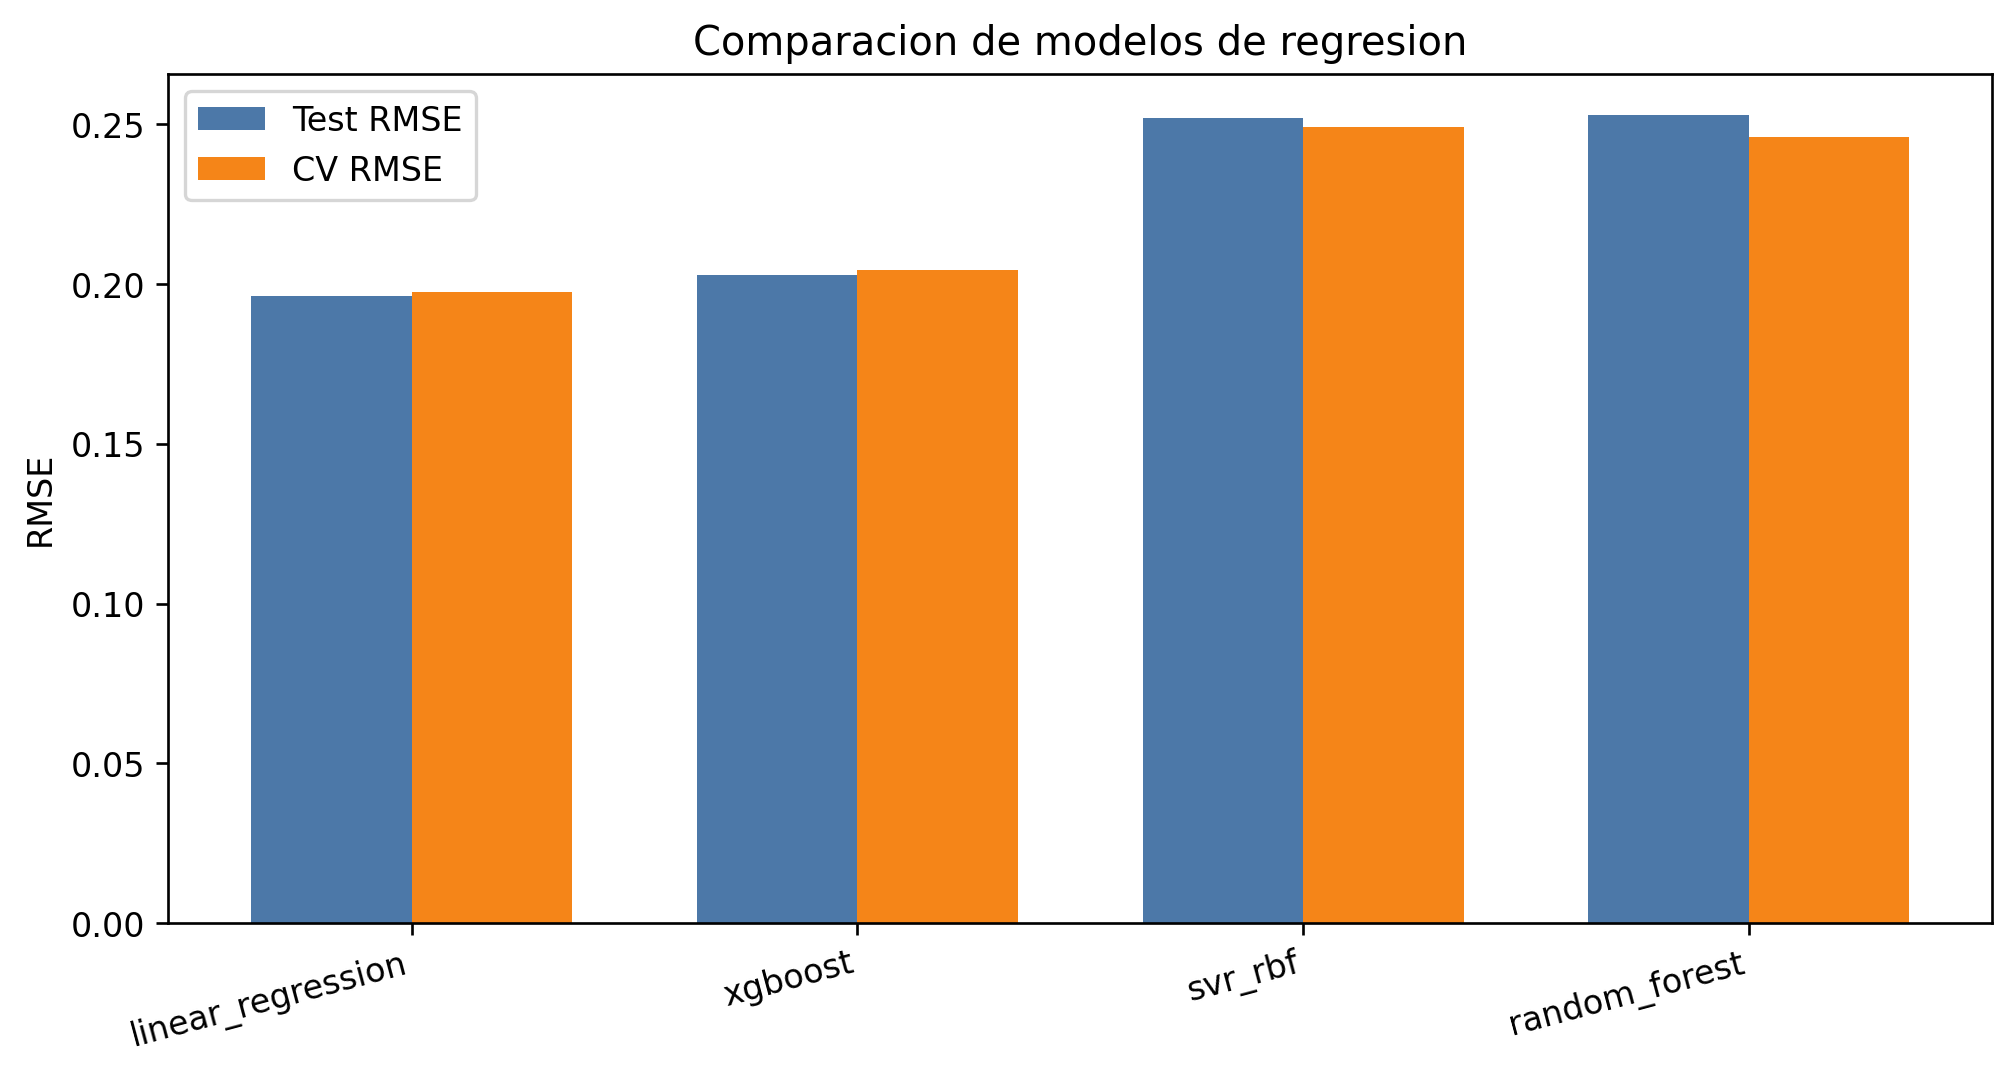
\includegraphics[width=\linewidth]{figures/fig_model_comparison.png}
\caption{Comparison of test and cross-validation RMSE.}
\label{fig:model_comparison}
\end{figure}

\begin{figure}[!t]
\centering
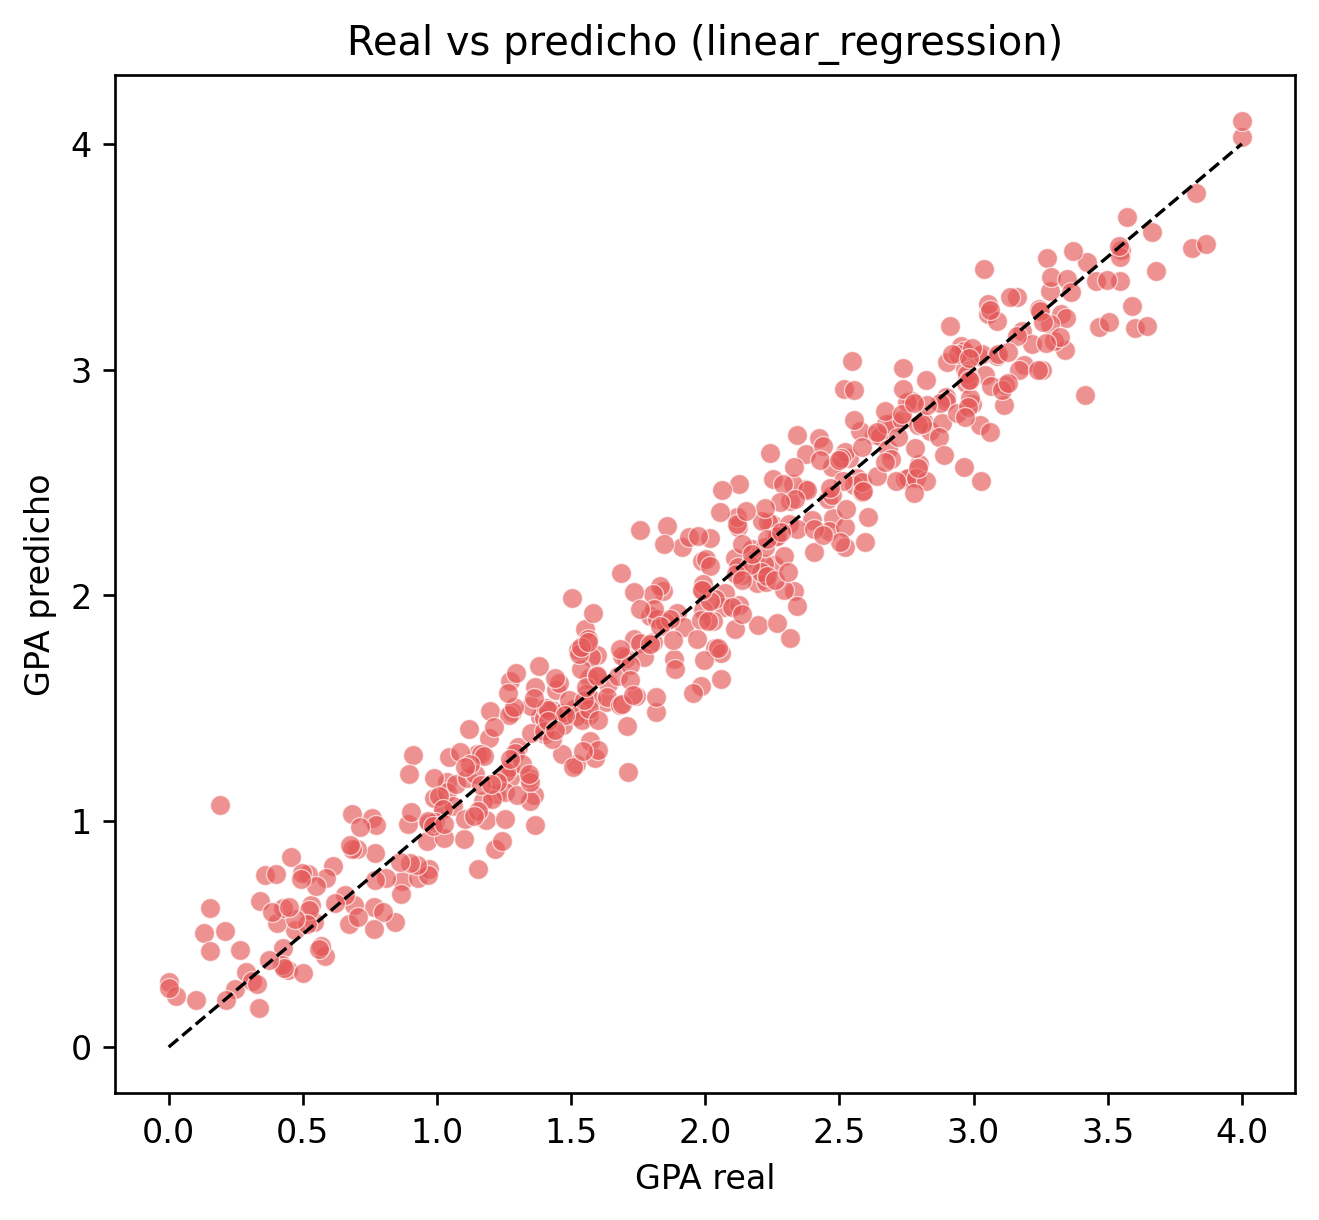
\includegraphics[width=\linewidth]{figures/fig_actual_vs_predicted.png}
\caption{Actual versus predicted values for the best regression model.}
\label{fig:actual_predicted}
\end{figure}

\subsection{XGBoost Case}

\begin{table}[!t]
\centering
\caption{Specific comparison between LinearRegression and XGBoost.}
\label{tab:xgboost}
\begin{tabular}{lrrrr}
\toprule
Model & Train RMSE & Test RMSE & Gap RMSE & Test $R^2$ \\
\midrule
LinearRegression & 0.1960 & 0.1963 & 0.0003 & 0.9534 \\
XGBoost & 0.1381 & 0.2117 & 0.0736 & 0.9458 \\
\bottomrule
\end{tabular}
\end{table}

XGBoost obtained lower RMSE on the training set, but not on the test set. This suggests that the model uses its higher flexibility to better fit the training data, but it does not improve generalization. The correlation between LinearRegression and XGBoost predictions was 0.9957, with a mean absolute difference of 0.0640. Therefore, XGBoost appears visually close to the linear model, but it is not the final best model.

\begin{figure}[!t]
\centering
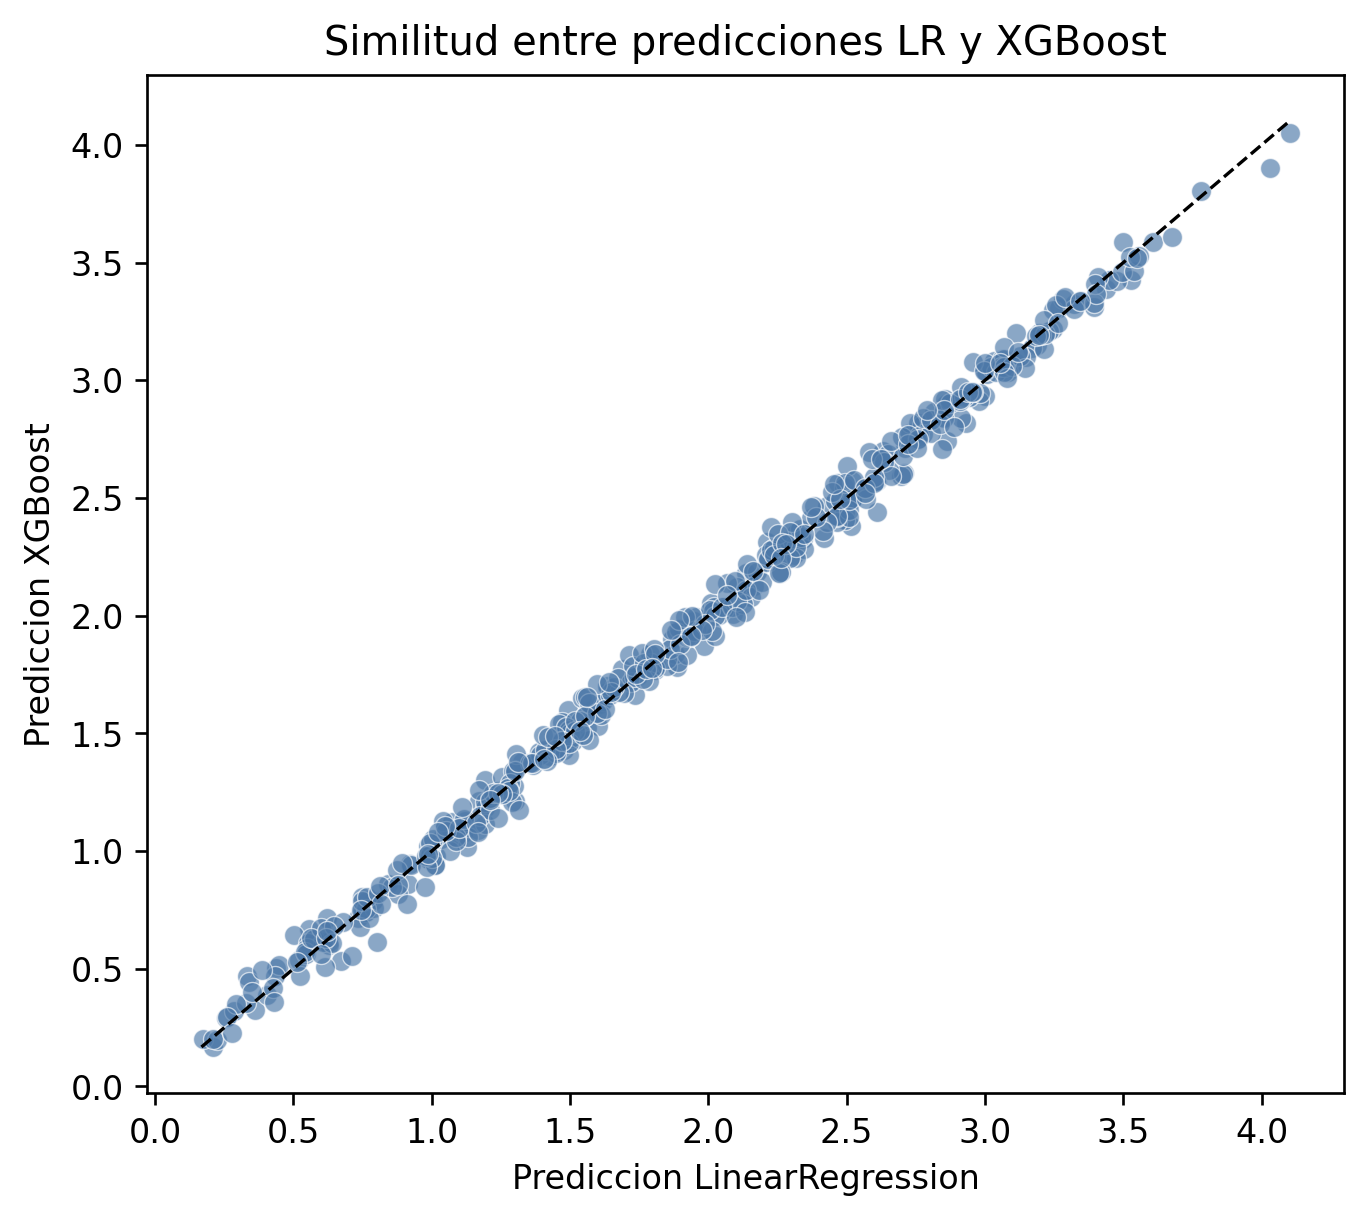
\includegraphics[width=\linewidth]{figures/fig_xgb_lr_predictions.png}
\caption{Direct comparison between LinearRegression and XGBoost predictions.}
\label{fig:xgb_lr}
\end{figure}

\subsection{Feature Importance and Absences Ablation}

Permutation importance showed that Absences is the dominant variable. Its mean importance was 1.0056 in RMSE increase when permuted, followed by ParentalSupport (0.1225), StudyTimeWeekly (0.1013), Tutoring (0.0519), and Sports (0.0413). The observed correlation between Absences and GPA was -0.9193.

\begin{figure}[!t]
\centering
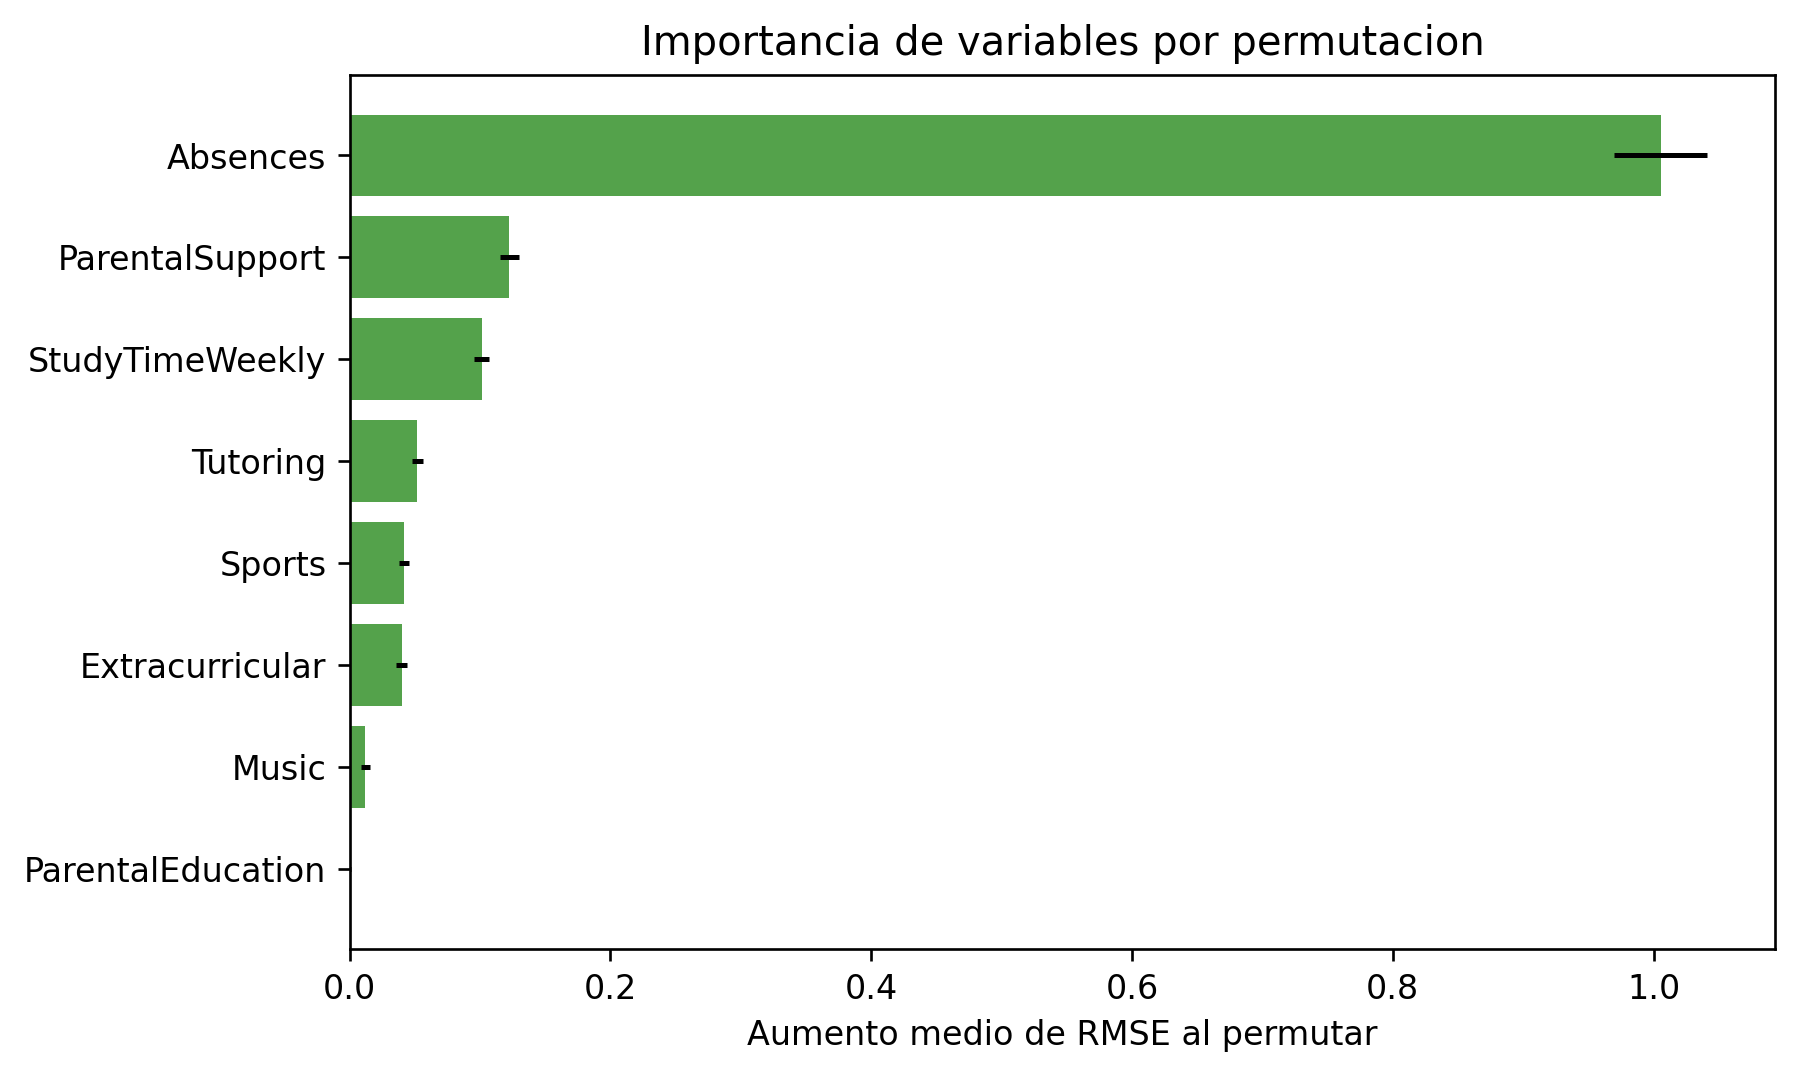
\includegraphics[width=\linewidth]{figures/fig_feature_importance.png}
\caption{Permutation feature importance on the test set.}
\label{fig:feature_importance}
\end{figure}

\begin{table}[!t]
\centering
\caption{Ablation test removing Absences.}
\label{tab:ablation}
\begin{tabular}{lrrrr}
\toprule
Model & Base RMSE & RMSE w/o Absences & $\Delta$ RMSE & $R^2$ w/o Absences \\
\midrule
LinearRegression & 0.1963 & 0.8692 & 0.6729 & 0.0864 \\
Random Forest & 0.2529 & 0.9278 & 0.6749 & -0.0411 \\
XGBoost & 0.2117 & 0.9398 & 0.7281 & -0.0681 \\
SVR RBF & 0.2520 & 1.0753 & 0.8233 & -0.3984 \\
\bottomrule
\end{tabular}
\end{table}

When Absences was removed, all models lost predictive capacity. In LinearRegression, RMSE increased from 0.1963 to 0.8692. This drop confirms that the main signal of the dataset is concentrated in absences.

\begin{figure}[!t]
\centering
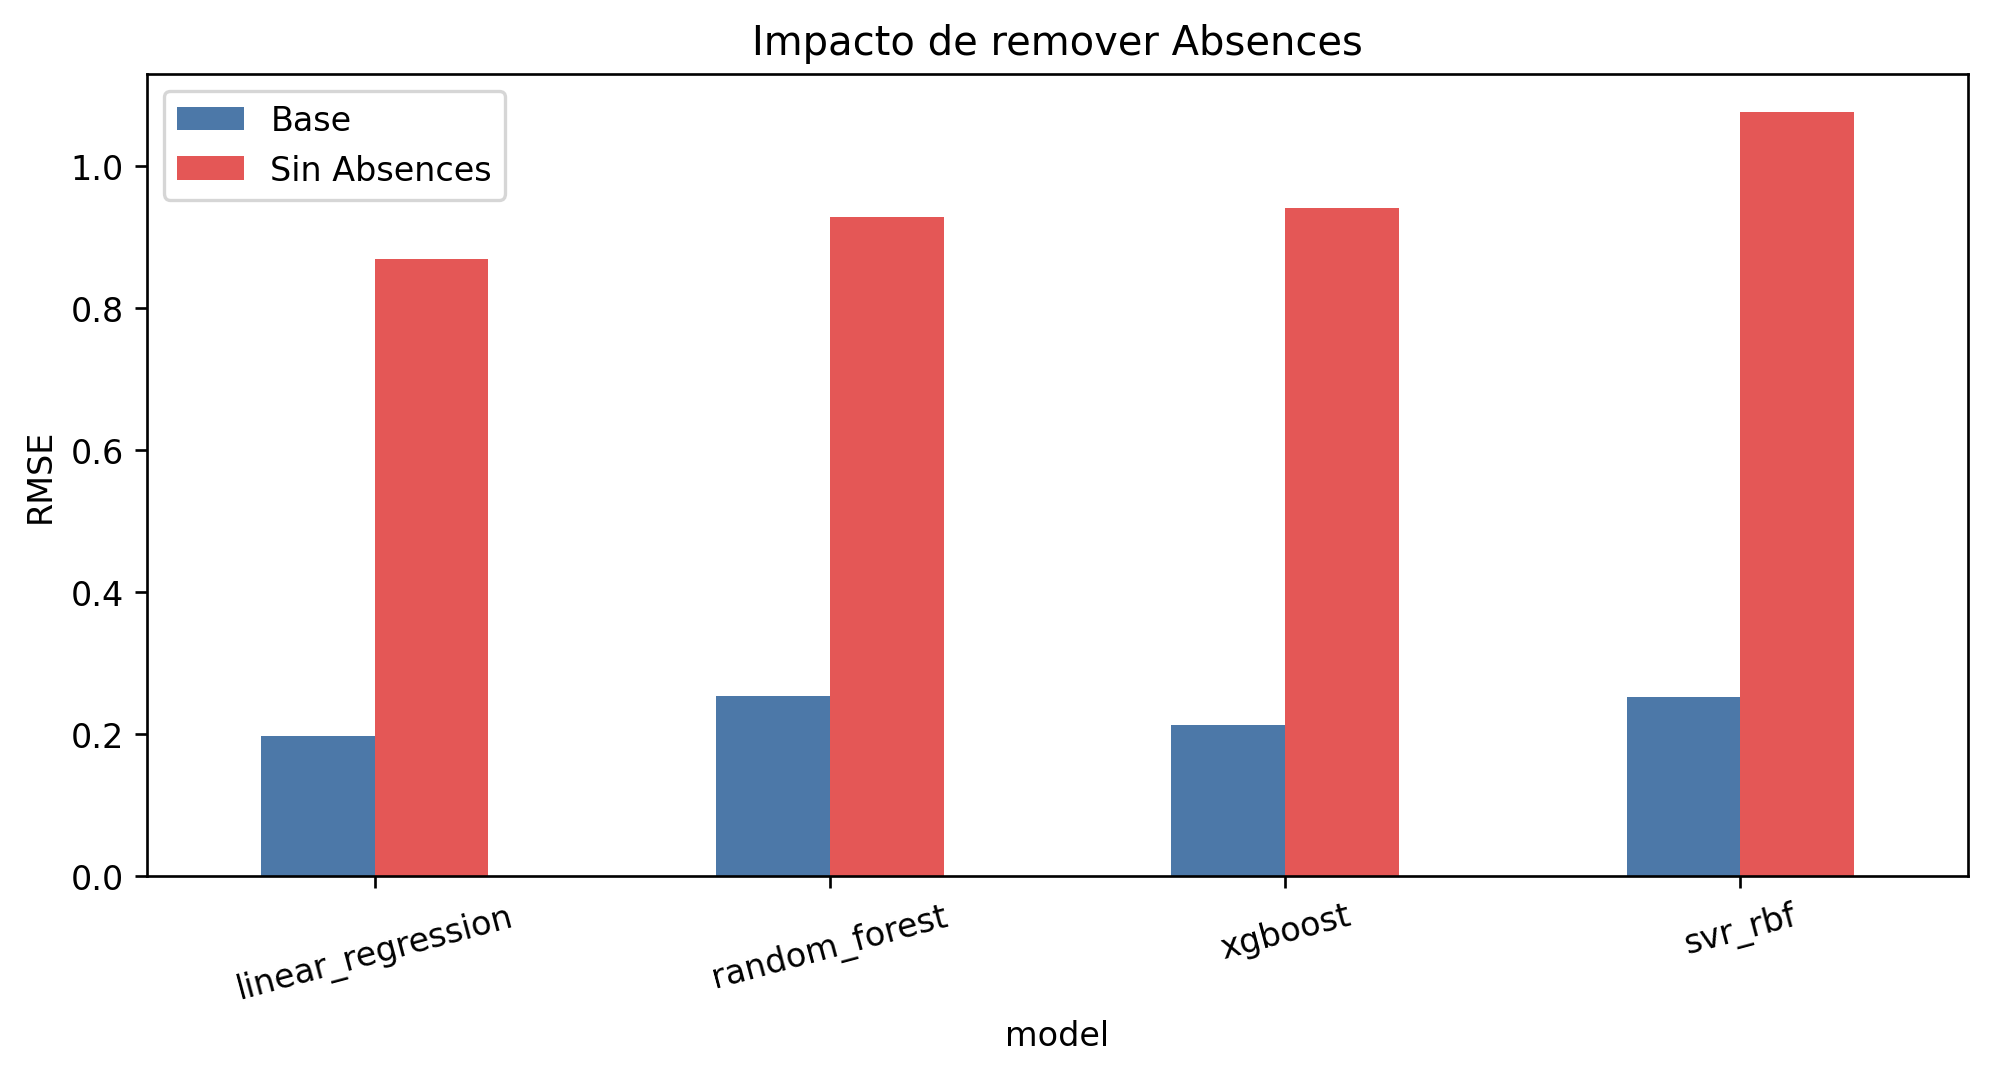
\includegraphics[width=\linewidth]{figures/fig_ablation_absences.png}
\caption{Effect of removing Absences on RMSE.}
\label{fig:ablation}
\end{figure}

\subsection{Good-Performance Classifier}

\begin{table}[!t]
\centering
\caption{Metrics of the calibrated good-performance classifier.}
\label{tab:classifier}
\begin{tabular}{lrrrr}
\toprule
Model & ROC AUC & Accuracy & F1 & Brier \\
\midrule
Calibrated LogisticRegression & 0.9871 & 0.9478 & 0.9110 & 0.0412 \\
\bottomrule
\end{tabular}
\end{table}

The calibrated classifier obtained ROC AUC = 0.9871, Average Precision = 0.9704, Accuracy = 0.9478, Precision = 0.9143, Recall = 0.9078, F1 = 0.9110, and Brier score = 0.0412. These results indicate that the model separates students who reach GPA $\geq 2.5$ from those below the threshold, and that its probabilities are useful for comparing scenarios.

\begin{figure}[!t]
\centering
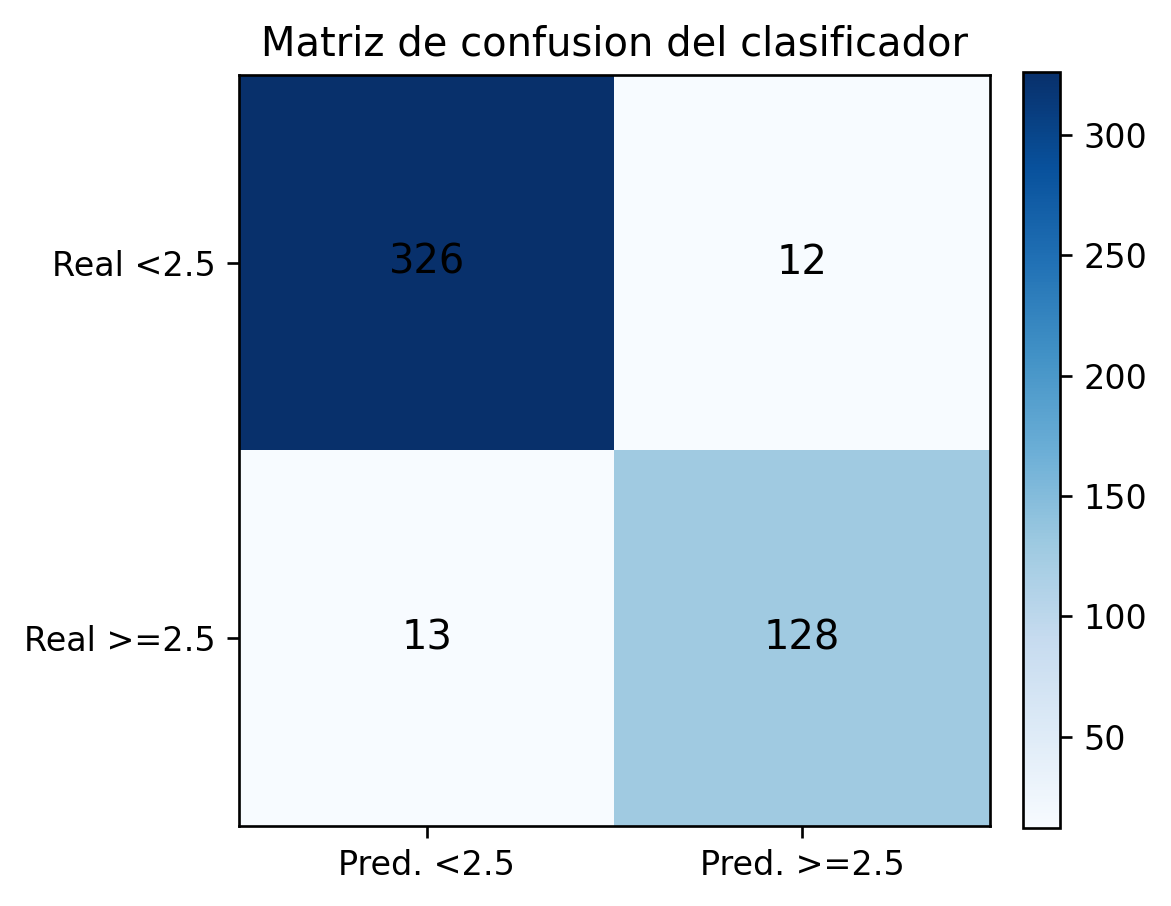
\includegraphics[width=\linewidth]{figures/fig_confusion_matrix.png}
\caption{Confusion matrix of the calibrated classifier.}
\label{fig:confusion}
\end{figure}

\begin{figure}[!t]
\centering
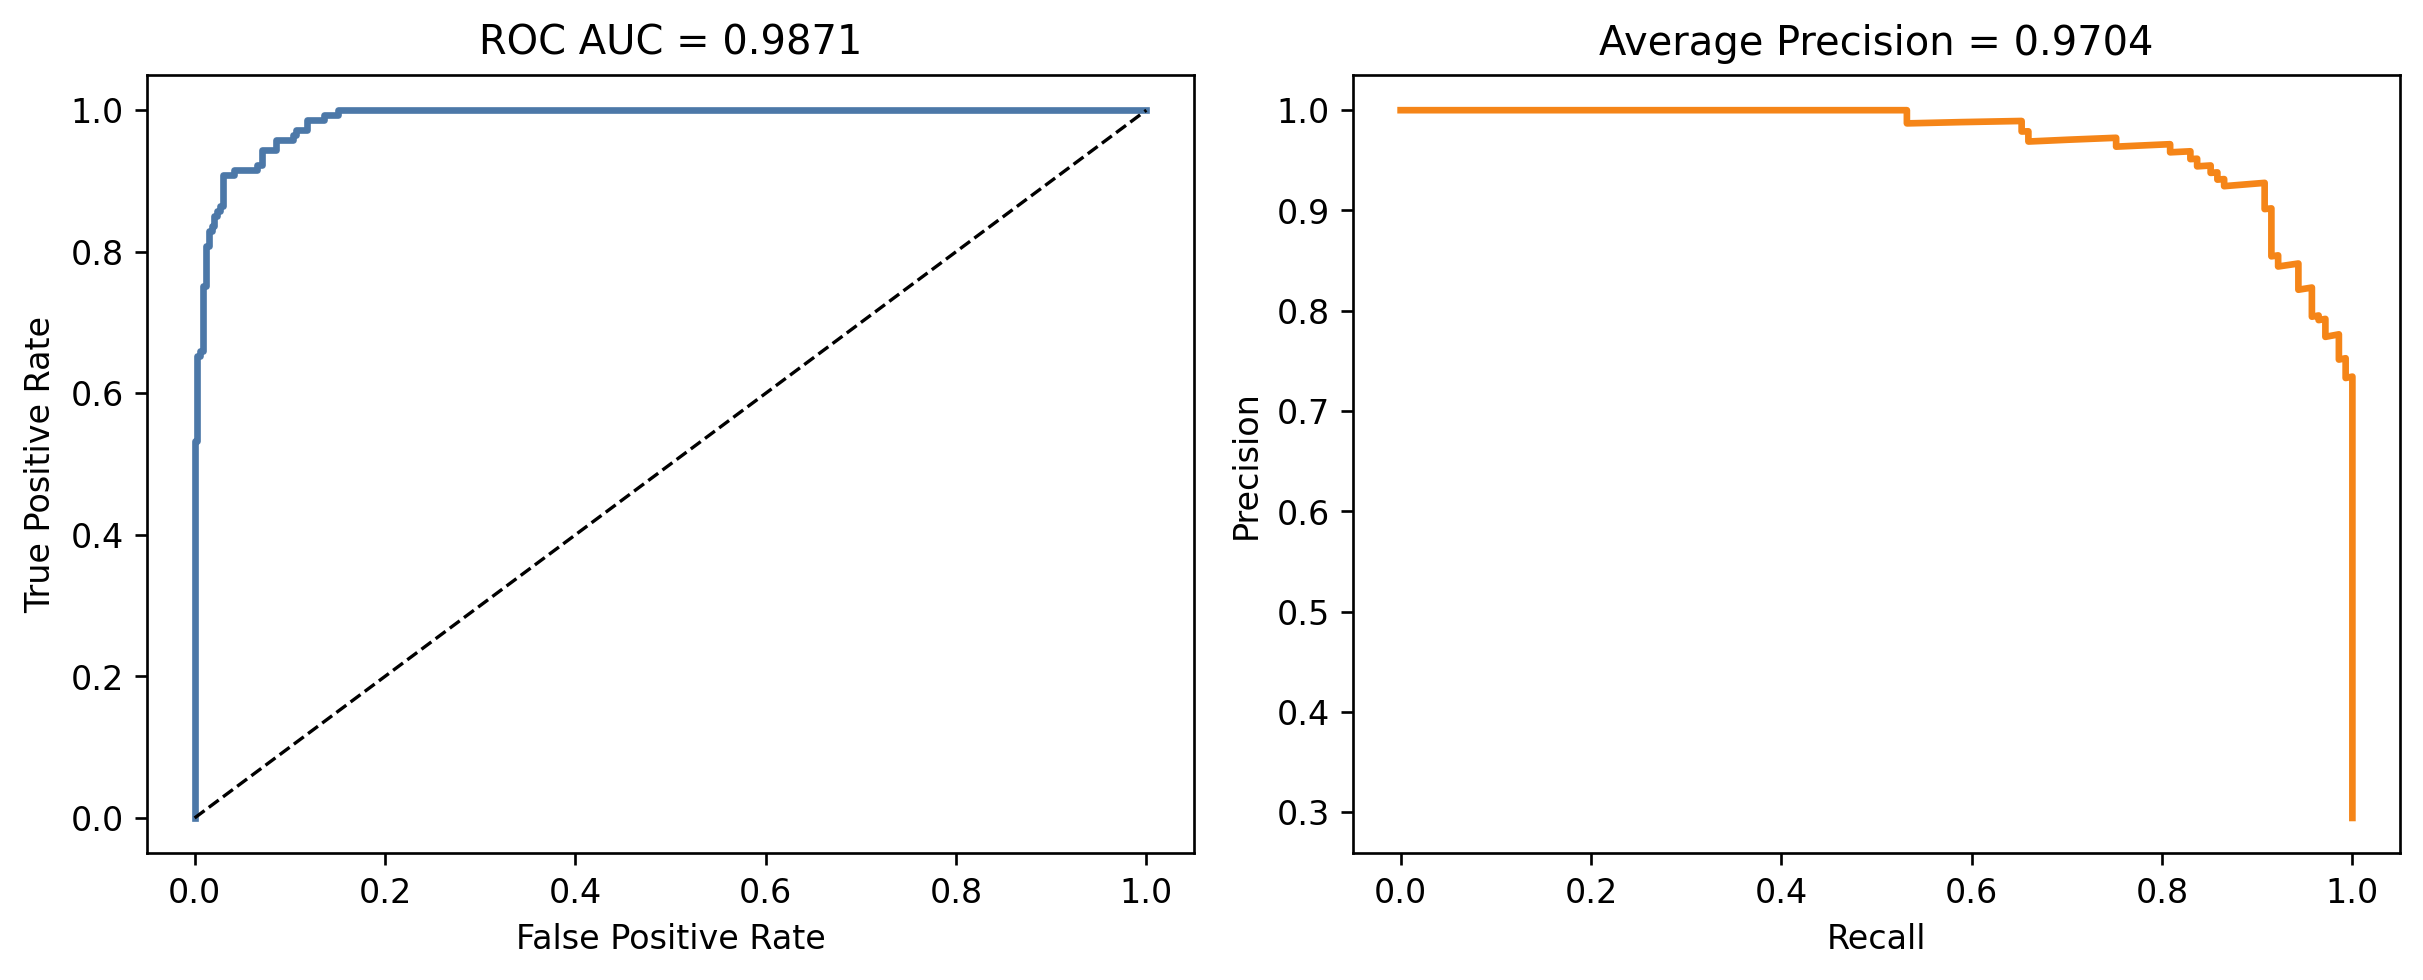
\includegraphics[width=\linewidth]{figures/fig_roc_pr_curves.png}
\caption{ROC and precision-recall curves of the calibrated classifier.}
\label{fig:roc_pr}
\end{figure}

\begin{figure}[!t]
\centering
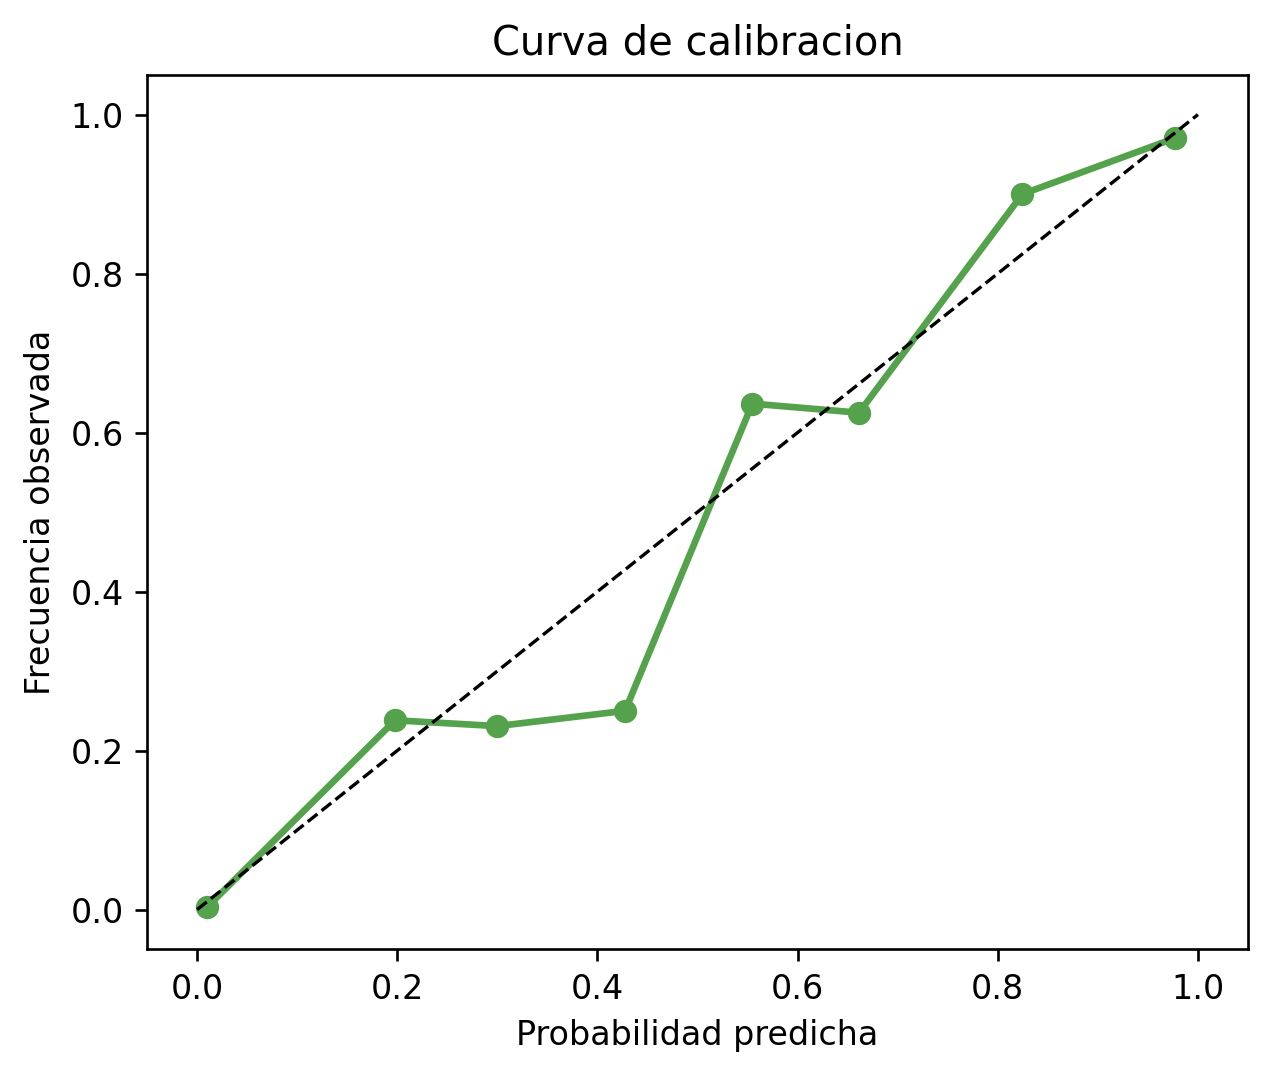
\includegraphics[width=\linewidth]{figures/fig_calibration_curve.png}
\caption{Probability calibration curve.}
\label{fig:calibration}
\end{figure}

\subsection{Student Recommendations}

For a high-risk case, the system recommended an intensive plan: reduce absences to a maximum of 5, increase study time up to 20 hours per week, enable tutoring, increase parental support by 2 levels, and enable an extracurricular activity. Under this simulation, the estimated GPA increased from 0.0000 to 3.6590, and the probability of good performance increased from approximately 0.0\% to 99.96\%. This result must not be interpreted as a causal guarantee, but as a simulation for prioritizing actions.

\begin{figure}[!t]
\centering
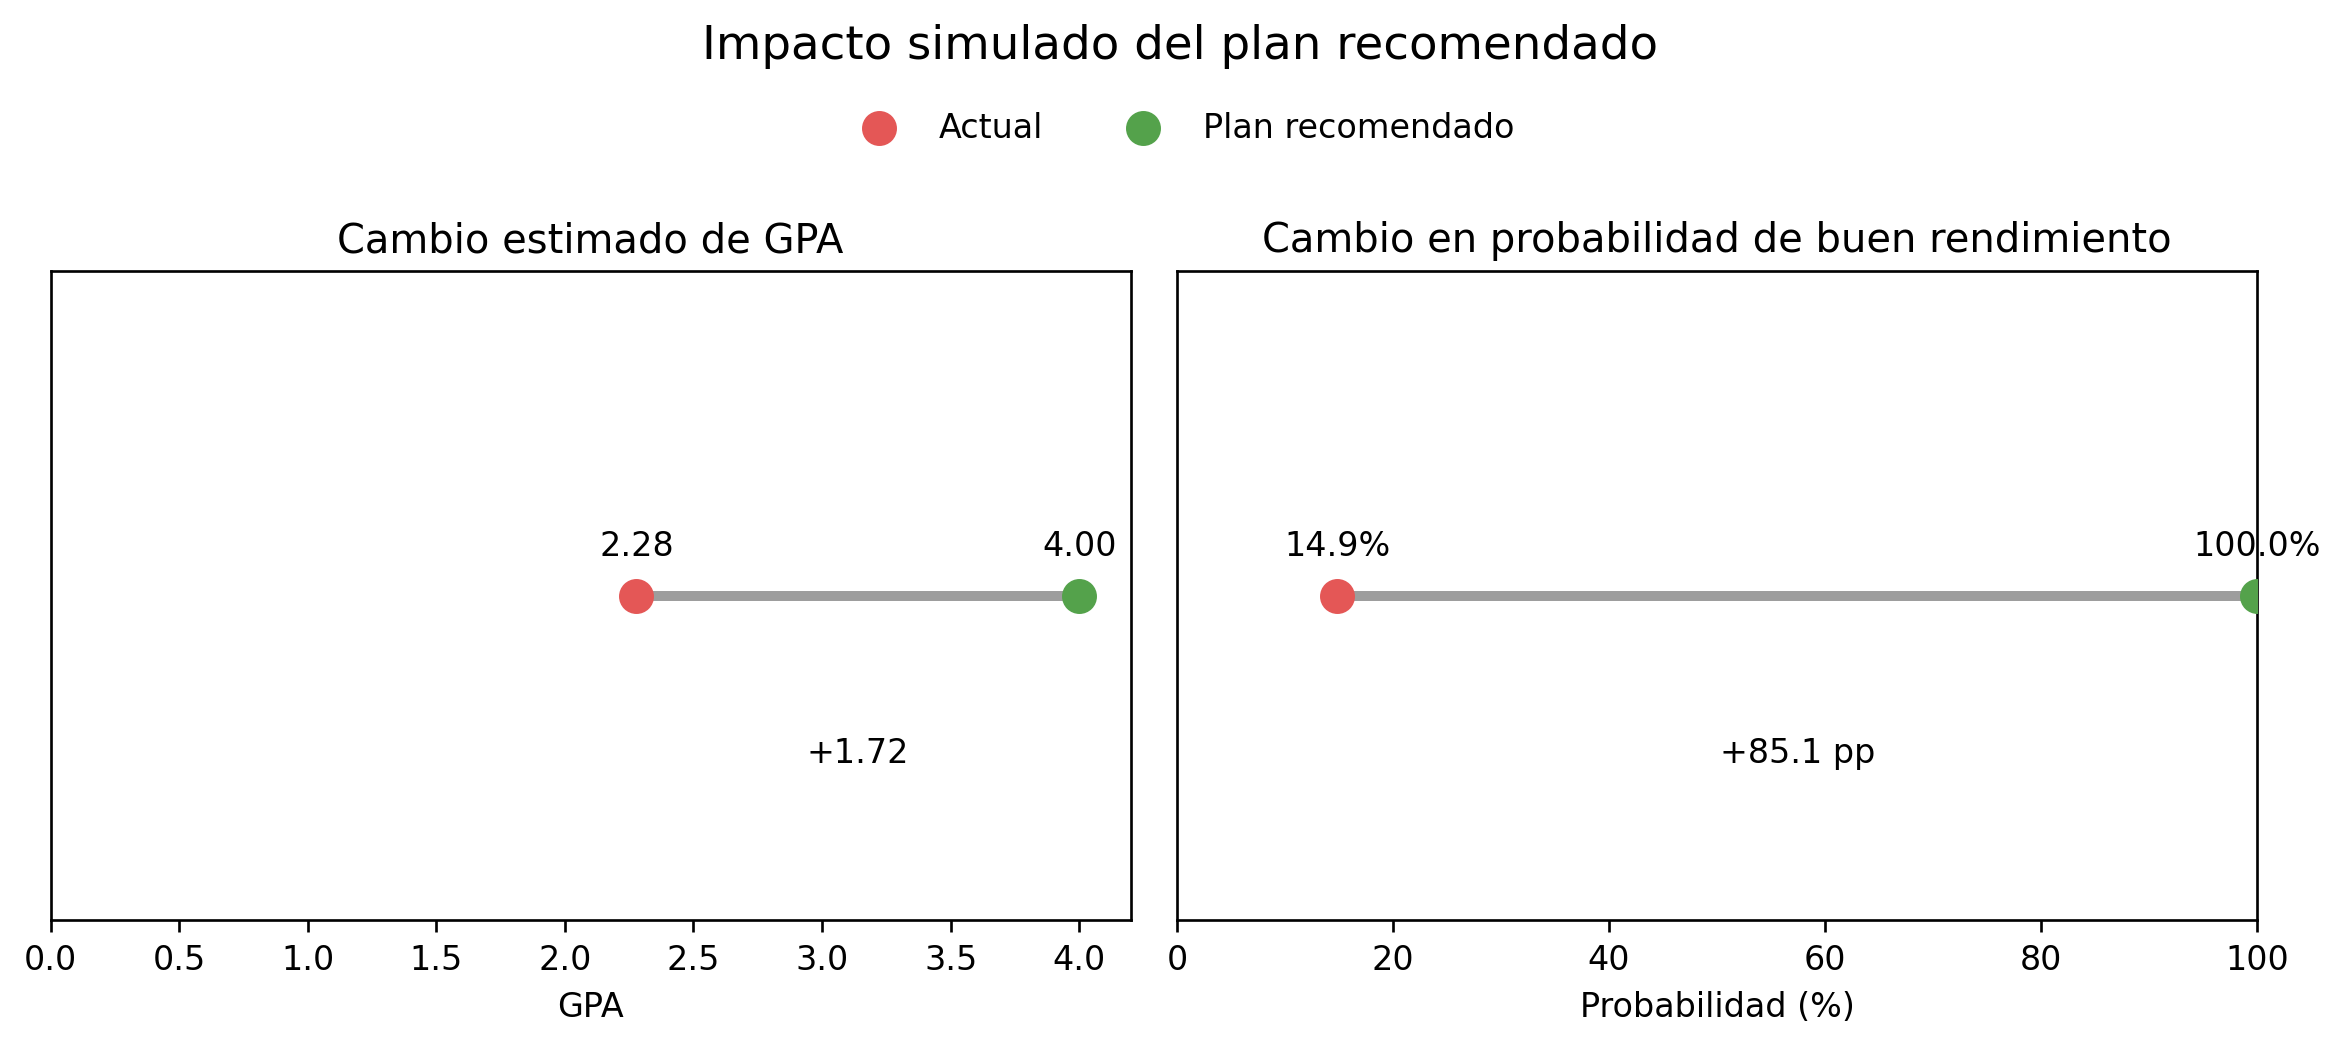
\includegraphics[width=\linewidth]{figures/fig_recommendation_plan.png}
\caption{Comparison between current scenario and recommended plan.}
\label{fig:recommendation}
\end{figure}

\subsection{Basic Fairness Audit}

Although Gender and Ethnicity are not used to recommend actions, group-level metrics were computed as a basic audit. In the test set, accuracy by Gender was 0.9375 for group 0 and 0.9582 for group 1. By Ethnicity, accuracy ranged from 0.9130 to 0.9637. These differences do not prove causal bias, but they justify subgroup monitoring before any school deployment.

\begin{figure}[!t]
\centering
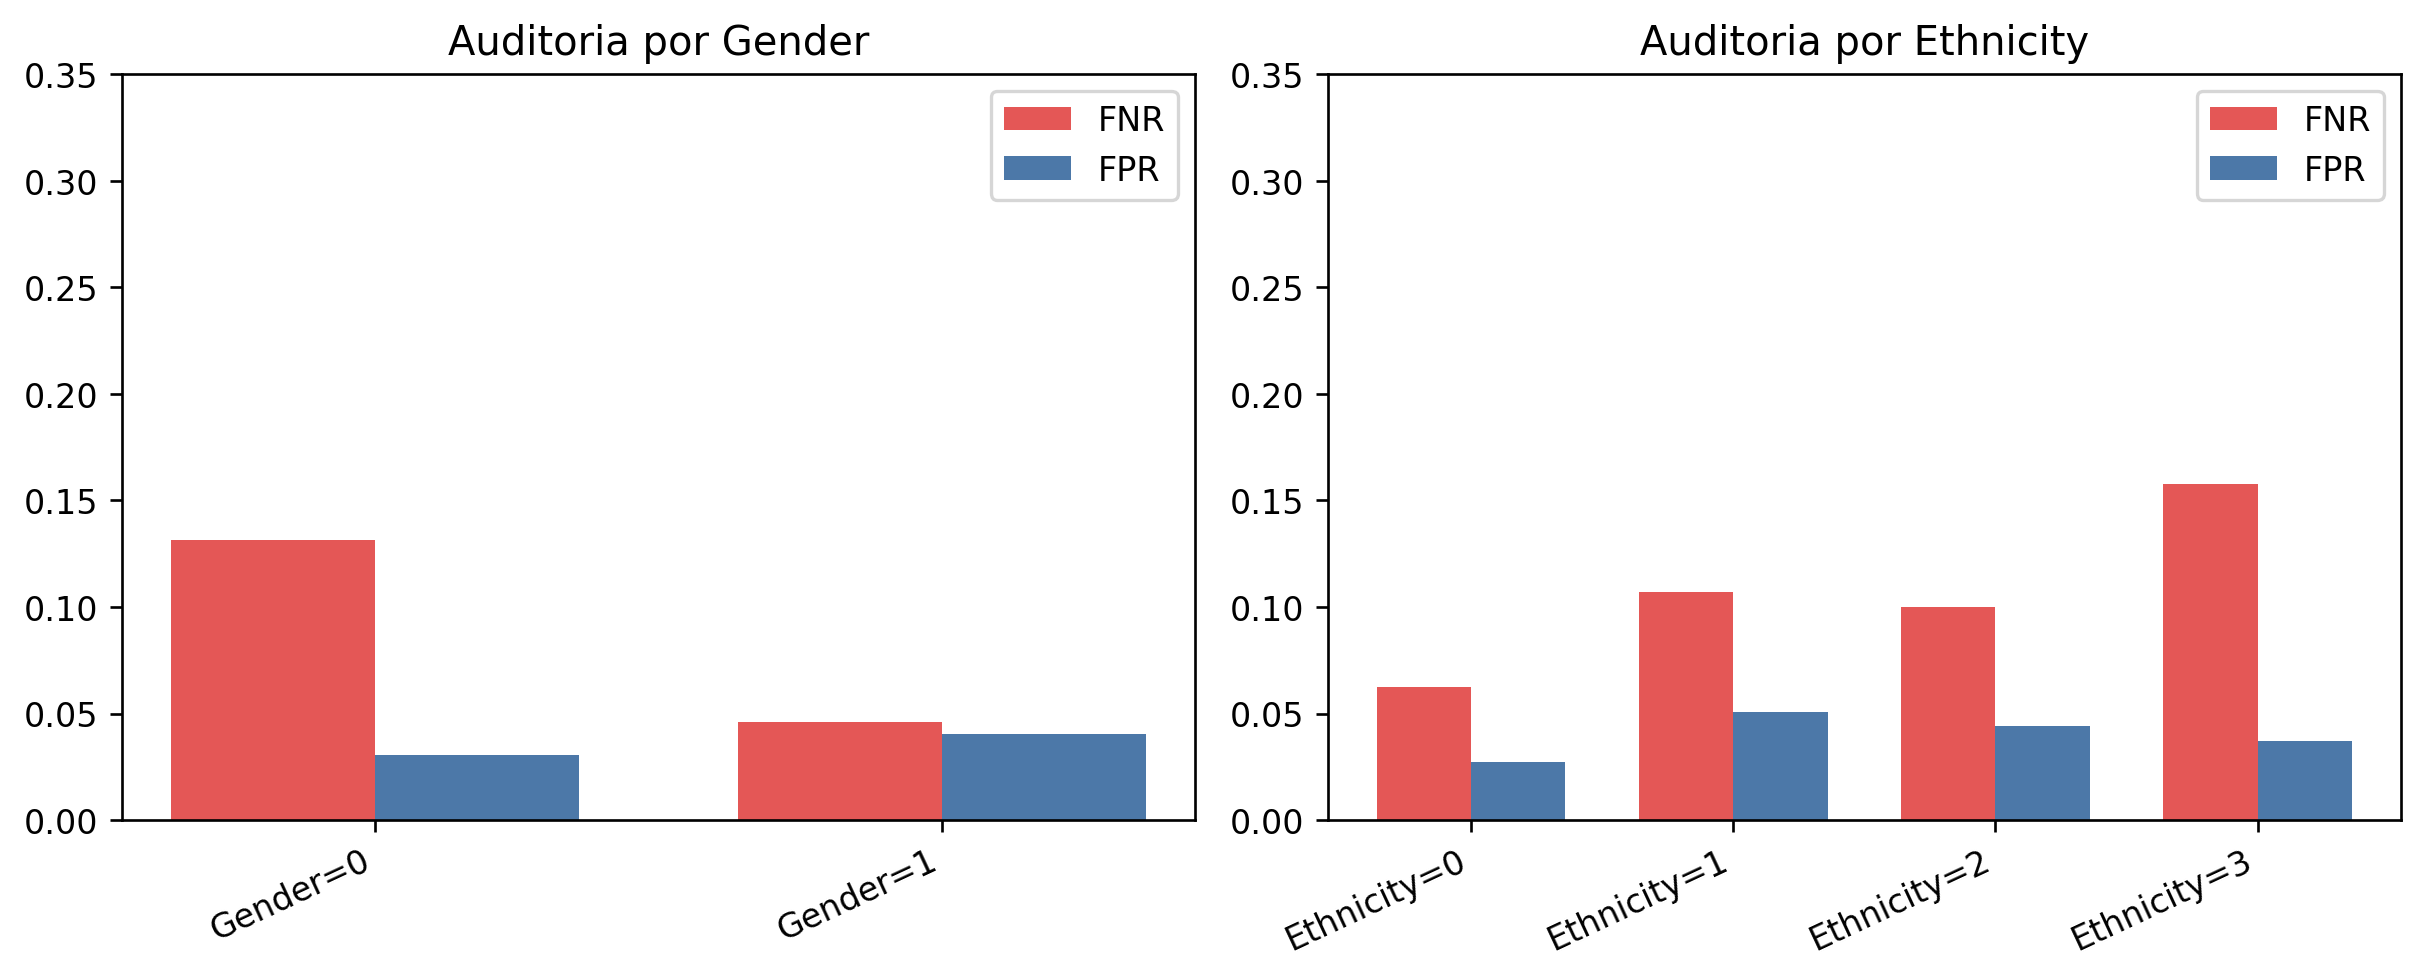
\includegraphics[width=\linewidth]{figures/fig_fairness_audit.png}
\caption{Exploratory audit by sensitive subgroups.}
\label{fig:fairness}
\end{figure}

\section{Discussion}

The results show that the most complex model was not necessarily the most appropriate. XGBoost has greater expressive capacity and fits the training set better, but the linear model generalizes better on the test set and cross-validation. This is consistent with the structure of the dataset: the dominant relationship between absences and GPA appears strong and nearly linear enough for a simple model to capture most of the signal.

The ablation test without Absences is the most important finding for educational interpretation. If that variable is removed, performance drops sharply. This has two implications. First, the model depends on a highly informative variable, so the system should not be presented as a general intelligence for school performance. Second, reducing absences is a priority intervention for at-risk students, although the model alone does not prove causality.

The recommendation component improves the usefulness of the project because it transforms predictive results into action scenarios. Instead of only displaying an estimated GPA, the system compares plans and quantifies the expected change. This layer turns the analysis into a potential support tool for tutors, coordinators, and students, as long as it is used as supervised support.

\section{Ethical Considerations and Limitations}

The system must not be used to sanction, exclude, or automatically label students. Its outputs are model-based simulations, not definitive academic decisions. In addition, although Gender and Ethnicity are excluded from the recommendation engine, the dataset may still contain historical biases or indirect relationships between variables. Therefore, institutional use would require periodic auditing, human review, and validation with local data.

There are several limitations. First, the dataset source should be fully documented before formal submission, even though the confirmed source is Kaggle \cite{kharoua2024students}. Second, the dataset is cross-sectional rather than longitudinal; therefore, the model does not estimate student evolution over time. Third, the recommendations are simple counterfactual simulations, not causal evidence. Fourth, relevant variables such as health, academic workload, socioeconomic conditions, teaching quality, and institutional context are not available. Fifth, the intensive demonstration plan maximizes performance under simulated rules, but its real feasibility depends on the student, tutor, and school.

\section{Conclusions}

This article presented a predictive and interpretable system for estimating GPA and generating actionable academic recommendations. The best regressor was LinearRegression, with RMSE = 0.1963 and $R^2$ = 0.9534 on the test set. XGBoost showed highly similar predictions, but with a larger train-test gap, so it was not selected as the final model. The ablation without Absences confirmed that absences are the most influential factor. The calibrated classifier achieved ROC AUC = 0.9871 and enabled the estimation of good-performance probabilities for comparing scenarios.

The practical contribution of the project is the connection between prediction and action: the system identifies risk factors, simulates improvement plans, and generates understandable messages to guide interventions. The next step is to turn the notebook into a school demo platform with CSV upload, individual student profiles, an intervention simulator, tutor reports, and ethical subgroup monitoring.

\section*{Availability}

The project repository is available at: \url{https://github.com/Edson-Zepeda/proyecto-gpa}. The paper figures and tables are generated using \texttt{paper/generate\_paper\_assets.py}.

\bibliographystyle{IEEEtran}
\bibliography{references}

\end{document}
